\usetikzlibrary{arrows.meta,calc,matrix,shapes}
\providecommand{\computer}{%
    
\includegraphics[width=1cm]{../common/Noun_project_216.pdf}
}
\providecommand{\switch}{%
    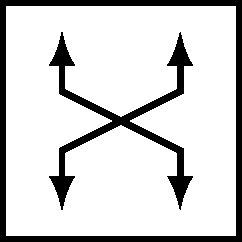
\includegraphics[width=0.9cm]{../common/fig-switch.pdf}
}
\providecommand{\router}{%
    
\includegraphics[width=0.9cm]{../common/fig-router.pdf}
}

\begin{frame}{spanning tree}
    \begin{itemize}
    \item given a general network, only activate subset of links
    \item \ldots such that network is tree
        \begin{itemize}
        \item that is only one path between each node
        \end{itemize}
    \vspace{.5cm}
    \item allows us to do flooding strategy
    \item makes simple MAC learning/broadcast just work
    \end{itemize}
\end{frame}

\begin{frame}{centralized spanning tree?}
    \begin{itemize}
    \item one algorithm you might learn in DSA2:
    \vspace{.5cm}
    \item mark one node called \textit{the root} as `in the tree'
    \item repeatedly: 
        \begin{itemize}
        \item add the `\myemph<2>{first}' link that goes to a node not in the tree
        \item mark newly connected node as `in the tree'
        \end{itemize}
    \vspace{.5cm}
    \item result = spanning tree
    \end{itemize}
\end{frame}

\begin{frame}{a careful ordering}
    \begin{itemize}
    \item algorithm works with any idea of which link/node is first
    \vspace{.5cm}
    \item we'll choose a particular ordering (for reasons you'll see later)
    \vspace{.5cm}
    \item first node one with earliest `name'
    \item links closer to the root before further links
    \item links from nodes with earlier names before later ones
    \end{itemize}
\end{frame}

\begin{frame}[fragile]{spanning tree example}
\begin{tikzpicture}
\tikzset{
    computer/.style={inner sep=0mm,outer sep=0mm,execute at begin node={\computer}},
    switch/.style={inner sep=0mm,outer sep=0mm,execute at begin node={\switch}},
    port/.style={pos=0.95,fill=white,circle,draw,inner sep=0mm},
    port beginning/.style={pos=0.05,fill=white,circle,draw,inner sep=0mm},
    route table/.style={
        matrix of nodes,ampersand replacement=\&,
        column 1/.style={nodes={draw,thick,text width=2.5cm,font=\tiny\tt,text depth=0mm,minimum height=0.5cm,inner sep=1mm}},
        column 2/.style={nodes={draw,thick,text width=.5cm,font=\small\tt,text depth=0mm,minimum height=0.5cm,inner sep=1mm}},
        row 1/.style={nodes={draw=none,font=\small}},
    },
    mac label/.style={
        draw,fill=white,inner sep=1mm,font=\tiny\tt,
    },
    tn/.style={draw,dotted,circle,very thick},
    real at/.style={alt=<#1->{solid},alt=<#1>{fill=red!10}},
    connect maybe/.style={draw,very thick,dotted,Latex-Latex},
    actual at/.style={alt=<#1->{draw=red,solid},alt=<#1>{draw,solid}},
    consider at/.style={alt=<#1>{draw=red}},
}
\node[tn,real at=1] (A) at (0, 0) {A};
\node[tn,real at=3] (B) at (5, -1) {B};
\node[tn,real at=4] (G) at (-5, -1) {G};
\node[tn,real at=6] (D) at (7, -3) {D};
\node[tn,real at=7] (E) at (1, -5) {E};
\node[tn,real at=8] (F) at (-7, -4) {F};
\draw[connect maybe,consider at=2,actual at=3] (A) -- (B)
    node[midway,sloped,above,visible on=<2>] {first priority};
\draw[connect maybe,consider at=2,actual at=4] (A) -- (G)
    node[midway,sloped,above,visible on=<2>] {second priority};
\draw[connect maybe,consider at=5] (B) -- (G)
    node[midway,sloped,below,visible on=<5>] {no new nodes};
\draw[connect maybe,actual at=6,consider at=5] (B) -- (D)
    node[midway,below left,visible on=<5>] {first priority};
\draw[connect maybe,actual at=8,consider at=5] (G) -- (F)
    node[midway,below right,visible on=<5>] {second priority};
\draw[connect maybe,consider at=6,actual at=7] (G) -- (E);
\draw[connect maybe,consider at=6] (D) -- (E);
\draw[connect maybe] (E) -- (F);
\end{tikzpicture}
\end{frame}

\begin{frame}{detecting `mistakes'}
    \begin{itemize}
    \item this method: consistent results every time
    \vspace{.5cm}
    \item but assumes we start from scratch
    \item we're going to want a way of doing this dynamically
    \vspace{.5cm}
    \item let's say we find a wrong configuration ---
    \item can we fix it?
    \end{itemize}
\end{frame}

\begin{frame}[fragile]{fixing wrong links}
\begin{tikzpicture}
\tikzset{
    computer/.style={inner sep=0mm,outer sep=0mm,execute at begin node={\computer}},
    switch/.style={inner sep=0mm,outer sep=0mm,execute at begin node={\switch}},
    port/.style={pos=0.95,fill=white,circle,draw,inner sep=0mm},
    port beginning/.style={pos=0.05,fill=white,circle,draw,inner sep=0mm},
    route table/.style={
        matrix of nodes,ampersand replacement=\&,
        column 1/.style={nodes={draw,thick,text width=2.5cm,font=\tiny\tt,text depth=0mm,minimum height=0.5cm,inner sep=1mm}},
        column 2/.style={nodes={draw,thick,text width=.5cm,font=\small\tt,text depth=0mm,minimum height=0.5cm,inner sep=1mm}},
        row 1/.style={nodes={draw=none,font=\small}},
    },
    mac label/.style={
        draw,fill=white,inner sep=1mm,font=\tiny\tt,
    },
    tn/.style={draw,dotted,circle,very thick},
    n real/.style={solid},
    n real at/.style={alt=<#1->{solid},alt=<#1>{fill=red!10}},
    n real until/.style={alt=<1-#1>{solid}},
    connect maybe/.style={draw,very thick,dotted,Latex-Latex},
    e real at/.style={alt=<#1>{draw=red,solid},alt=<#1->{draw,solid}},
    e real until/.style={alt=<1-#1>{solid},alt=<#1>{draw=red,solid}},
    e real/.style={solid},
    e hide up to/.style={alt=<1-#1>{invisible}},
    consider at/.style={alt=<#1>{draw=red,dotted}},
    explain box/.style={at={(0, -4)},align=center,draw=red,ultra thick,fill=white},
    explain box up/.style={at={(2, -1)},align=center,draw=red,ultra thick,fill=white},
}
\node[tn,n real] (A) at (0, 0) {A};
\node[tn,n real] (B) at (5, -1) {B};
\node[tn,n real] (G) at (-5, -1) {G};
\node[tn,n real] (D) at (7, -3) {D};
\node[tn,n real] (E) at (1, -5) {E};
\node[tn,n real] (F) at (-7, -4) {F};
\draw[connect maybe,e real] (A) -- (B);
\draw[connect maybe,e hide up to=1,e real at=2,consider at=2,alt=<3->{draw=black}] (A) -- (G);
\draw[connect maybe,e real until=2] (B) -- (G);
\draw[connect maybe,e real] (B) -- (D);
\draw[connect maybe,e real] (G) -- (F);
\draw[connect maybe,e hide up to=4,e real at=5] (G) -- (E);
\draw[connect maybe,e hide up to=2,alt=<3-4>{solid},alt=<3>{red},alt=<5>{red}] (D) -- (E);
\draw[connect maybe,e real until=3] (E) -- (F);
\begin{visibleenv}<2>
\node[explain box] {
    A--G beats B--G: closer to root
};
\end{visibleenv}
\begin{visibleenv}<3>
\node[explain box up] {
    D--F and F--E: \\
    same distance from root, but \\
    D before F, so D--E beats F--E
};
\end{visibleenv}
\begin{visibleenv}<5>
\node[explain box up] {
    G--E and D--E: \\
    G--E closer to root \\
    so G--E beats D--E
};
\end{visibleenv}
\end{tikzpicture}
\end{frame}

\begin{frame}{spanning tree protocol}
    \begin{itemize}
    \item each node tracks:
        \begin{itemize}
        \item what it believes is root of tree
        \item its link toward root of tree
        \item its distance to root of tree
        \item which other nodes think it's closer to root of tree
        \end{itemize}
    \item periodically sends information to neighbors
    \item when receiving information, update:
        \begin{itemize}
        \item root to lower ID number (if possible)
        \item link to lower-distance link  (if possible)
        \item link to lower-ID, same-distance link (if possible)
        \item which other nodes think it is closer
        \end{itemize}
    \end{itemize}
\end{frame}

\begin{frame}[fragile]{some example updates}
\begin{tikzpicture}
\tikzset{
    computer/.style={inner sep=0mm,outer sep=0mm,execute at begin node={\computer}},
    switch/.style={inner sep=0mm,outer sep=0mm,execute at begin node={\switch}},
    port/.style={pos=0.95,fill=white,circle,draw,inner sep=0mm},
    port beginning/.style={pos=0.05,fill=white,circle,draw,inner sep=0mm},
    route table/.style={
        matrix of nodes,ampersand replacement=\&,
        column 1/.style={nodes={draw,thick,text width=2.5cm,font=\tiny\tt,text depth=0mm,minimum height=0.5cm,inner sep=1mm}},
        column 2/.style={nodes={draw,thick,text width=.5cm,font=\small\tt,text depth=0mm,minimum height=0.5cm,inner sep=1mm}},
        row 1/.style={nodes={draw=none,font=\small}},
    },
    mac label/.style={
        draw,fill=white,inner sep=1mm,font=\tiny\tt,
    },
    n real/.style={solid},
    n real at/.style={alt=<#1->{solid},alt=<#1>{fill=red!10}},
    n real until/.style={alt=<1-#1>{solid}},
    tn/.style={draw,dotted,circle,very thick},
    real at/.style={alt=<#1->{solid},alt=<#1>{fill=red!10}},
    connect maybe/.style={draw,very thick,dotted,Latex-Latex},
    actual at/.style={alt=<#1->{draw=red,solid},alt=<#1>{draw,solid}},
    consider at/.style={alt=<#1>{draw=red}},
    msg link/.style={draw,violet,line width=1.2mm,-Latex},
    msg data/.style={draw=violet,line width=1mm,fill=white,align=left},
}
\node[tn,n real] (A) at (0, 0) {A};
\node[tn,n real] (B) at (5, -1) {B};
\node[tn,n real] (G) at (-5, -1) {G};
\node[tn,n real] (D) at (7, -3) {D};
\node[tn,n real] (E) at (1, -5) {E};
\node[tn,n real] (F) at (-7, -4) {F};
\draw[connect maybe] (A) -- (B);
\draw[connect maybe] (A) -- (G);
\draw[connect maybe] (B) -- (G);
\draw[connect maybe] (B) -- (D);
\draw[connect maybe] (G) -- (F);
\draw[connect maybe] (G) -- (E);
\draw[connect maybe] (D) -- (E);
\draw[connect maybe] (E) -- (F);
\tikzset{
    every node/.style={font=\small},
}
\begin{visibleenv}<2>
    \draw[msg link] (E) -- (G);
    \draw[msg link] (E) -- (F);
    \draw[msg link] (E) -- (D);
    \node[draw,very thick,anchor=south west] at (G.north east) {
        r=G,d=0,no link
    };
    \node[draw,very thick,alt=<2>{msg data},anchor=north] at (E.south) {
        r=E,d=0,no link
    };
    \node[draw,very thick,anchor=north west] at (F.south east) {
        r=F,d=0,no link
    };
    \node[draw,very thick,anchor=north west] at (D.south west) {
        r=D,d=0,no link
    };
\end{visibleenv}
\begin{visibleenv}<3>
    \draw[msg link] (E) -- (G);
    \draw[msg link] (E) -- (F);
    \draw[msg link] (E) -- (D);
    \node[draw,very thick,draw=red,anchor=south west] at (G.north east) {
        r=E,d=1,G--E
    };
    \node[draw,very thick,anchor=north] at (E.south) {
        r=E,d=0,no link
    };
    \node[draw,very thick,draw=red,anchor=north west] at (F.south east) {
        r=E,d=0,F--E
    };
    \node[align=left,draw,very thick,draw=red,anchor=north east] at (D.south west) {
        r=D,d=0,no link \\
        (D < G, so no update)
    };
\end{visibleenv}
\begin{visibleenv}<4>
    \draw[msg link] (D) -- (B);
    \draw[msg link] (D) -- (E);
    \node[draw,very thick,anchor=south west] at (G.north east) {
        r=E,d=1,G--E
    };
    \node[draw,very thick,anchor=north] at (E.south) {
        r=E,d=0,no link
    };
    \node[draw,very thick,anchor=north west] at (F.south east) {
        r=E,d=0,F--E
    };
    \node[draw,very thick,alt=<4>{msg data},anchor=north east] at (D.south west) {
        r=D,d=0,no link
    };
    \node[draw,very thick,anchor=south] at (B.north) {
        r=B,d=0,no link
    };
\end{visibleenv}
\begin{visibleenv}<5>
    \draw[msg link] (D) -- (B);
    \draw[msg link] (D) -- (E);
    \node[draw,very thick,anchor=south west] at (G.north east) {
        r=E,d=1,G--E
    };
    \node[draw,very thick,draw=red,anchor=north] at (E.south) {
        r=D,d=1,E--D
    };
    \node[draw,very thick,anchor=north west] at (F.south east) {
        r=E,d=0,F--E
    };
    \node[draw,very thick,anchor=north east] at (D.south west) {
        r=D,d=0,no link
    };
    \node[align=left,draw,very thick,draw=red,anchor=south] at (B.north) {
        r=B,d=0,no link \\
        (B < D, no update)
    };
\end{visibleenv}
\end{tikzpicture}
\end{frame}

\begin{frame}{spanning trees in practice (1)}
    \begin{itemize}
    \item commonly used on Ethernet for switches
    \item links not in spanning tree are `blocked'
        \begin{itemize}
        \item not used for normal traffic
        \item assumption: would cause loop $\rightarrow$ infinite packets
        \end{itemize}
    \item delay before activating port
        \begin{itemize}
        \item avoid temporary routing loops while figuring out tree
        \end{itemize}
    \item periodically send updates to all neighbors
        \begin{itemize}
        \item order of seconds
        \end{itemize}
    \end{itemize}
\end{frame}

\begin{frame}{spanning tree in practice (2)}
    \begin{itemize}
    \item real protocol supports variable `cost' for links
        \begin{itemize}
        \item so `distance to root' might be lower for faster links
        \end{itemize}
    \item modern variant (Rapid Spanning Tree Protocol) selects ``backup'' port to root 
        \begin{itemize}
        \item goal: faster switchover on failure
        \end{itemize}
    \end{itemize}
\end{frame}
